\section{Proposed Method}

\subsection{The DeepLab CNN + CRF Model for Semantic Image Segmentation}

Our starting point is the recently proposed DeepLab model for semantic
image segmentation \cite{chen2014semantic}, illustrated in
Figure~\ref{fig:model_test}. This model applies a deep CNN in a
sliding window fashion to generate for each image dense segmentation
score maps 
\begin{equation}
  \label{eq:scores}
  f_i(x_i; \theta) \,,
  \quad \mathrm{with} \quad
  P_i(x_i; \theta) \propto \exp \left( f_i(x_i; \theta) \right)
\end{equation}
where $x_i \in \mathcal{L}$ is the assignment of the $i$-th pixel to
the discrete candidate semantic label set $\mathcal{L}$, $\theta$
is the vector of CNN model parameters, and normalization ensures
that $\sum_{l \in \mathcal{L}} P_i(l; \theta) = 1$. Score map
post-processing by means of a fully-connected CRF (Dense CRF)
\cite{krahenbuhl2011efficient} significantly improves segmentation
performance near object boundaries. Computation sharing in the
convolutional layers by means of the hole algorithm and careful
network crafting make the method computationally efficient.

\begin{figure}[htbp!]
  \centering
  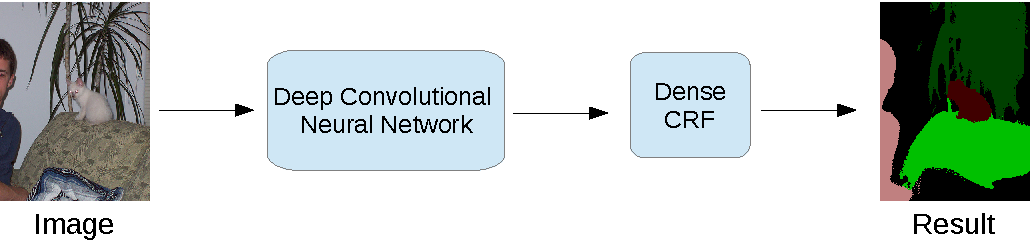
\includegraphics[width=0.9\linewidth]{fig/model_test.pdf} 
  \caption{Overview of the DeepLab CNN + CRF semantic segmentation model.}
  \label{fig:model_test}
\end{figure}

\subsection{Model Training on Fully Annotated Images}
\label{sec:train_pixel}

The network parameters $\theta$ are initialized from an
Imagenet-pretrained deep CNN model \cite{simonyan2014very} and
fine-tuned by stochastic gradient descent so as to minimize the
average log-loss 
\begin{equation}
  \label{eq:log_loss}
  L(\theta) = \frac{1}{N} \sum_{i = 1}^N \log P_i(l_i; \theta)
\end{equation}
between the model predictions and the pixel-wise ground truth
labels $\{l_i\}_{i = 1}^N$, as illustrated in
Figure~\ref{fig:model_train_pixel}. Similarly to
\cite{chen2014semantic}, we do not include the Dense CRF module into
the training pipeline for simplicity and speed during training.

Learning the DeepLab model on fully annotated images works very well
in practice, yielding excellent performance (66.4 \% IoU) in the
challenging PASCAL VOC 2012 image segmentation benchmark. However, the
need for such detailed annotations makes it harder to gather very
large training datasets and makes it difficult to train the model
for new domains, especially when the number of candidate labels
(cardinality of the label set $\mathcal{L}$) is big.

\begin{figure}[htbp!]
  \centering
  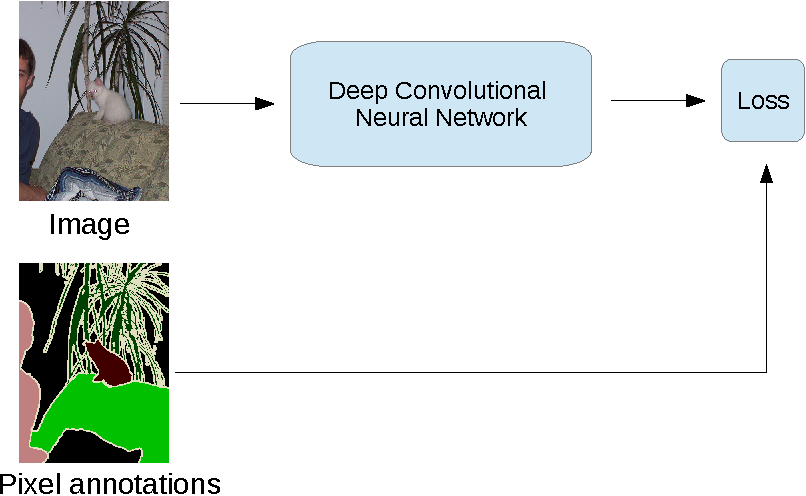
\includegraphics[width=0.9\linewidth]{fig/model_train_pixel.pdf} 
  \caption{DeepLab model training from fully annotated images.}
  \label{fig:model_train_pixel}
\end{figure}

\subsection{Model Training on Weak Bounding Box Annotated Images}
\label{sec:train_bbox}

Collecting bounding box annotations is significantly easier compared
to pixel-level ground truth segmentations. We have explored two
methods for training the DeepLab segmentation model from bounding
boxes with object-level labels. In both methods we estimate dense
segmentation maps from the bounding box annotation as a pre-processing
step, then employ the training procedure of
Section~\ref{sec:train_pixel} treating these estimated labels as
ground-truth.

The first baseline method amounts to simply considering each pixel
within the bounding box as positive example for the respective object
class. Ambiguities are resolved by assigning pixels that belong to
multiple bounding boxes to the one that has the smallest area.

\emph{GRABCUT GOES HERE}

\begin{figure}[htbp!]
  \centering
  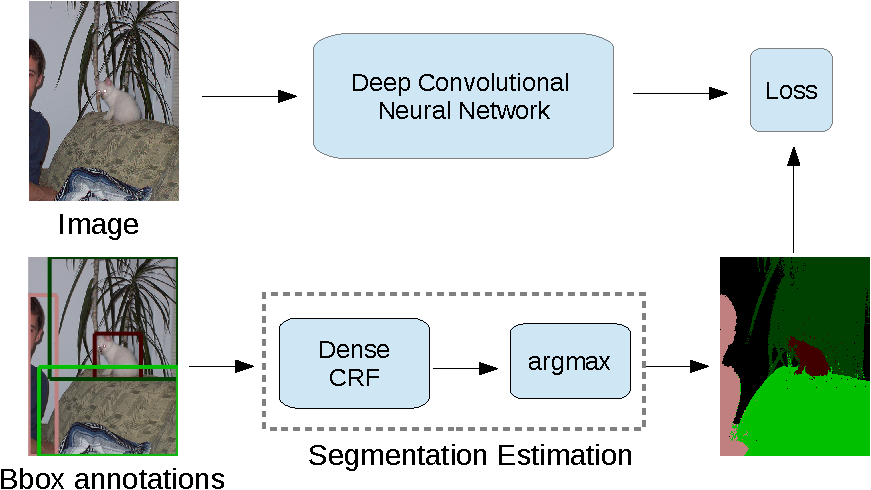
\includegraphics[width=0.9\linewidth]{fig/model_train_bbox.pdf} 
  \caption{DeepLab model training using bounding box data and
    automated foreground/ background segmentation.}
  \label{fig:model_train_bbox}
\end{figure}


\subsection{Model Training Using Weak Image-Level Labels}



\begin{figure}[htbp!]
  \centering
  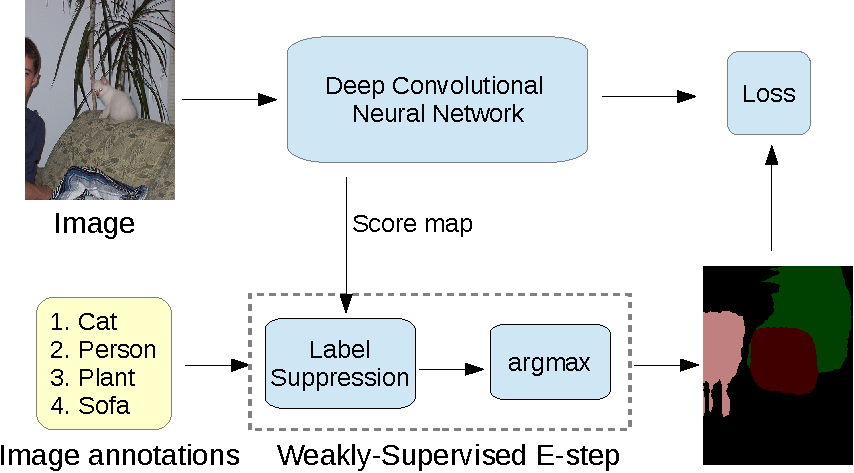
\includegraphics[width=0.9\linewidth]{fig/model_train_image.pdf} 
  \caption{DeepLab model training using image-level labels by
    censored Expectation-Maximization.}
  \label{fig:model_train_image}
\end{figure}

\subsection{Model Training on a Combination of Fully and Weakly Annotated Images}

\begin{figure}[htbp!]
  \centering
  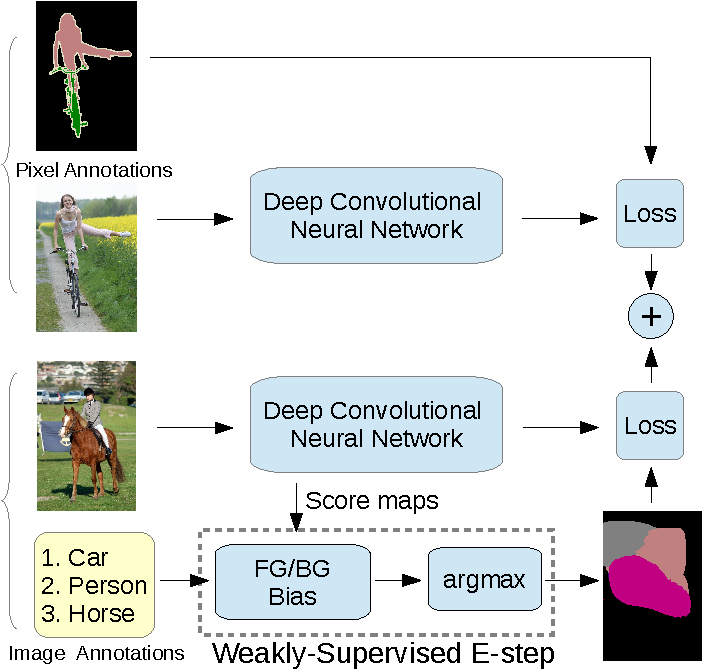
\includegraphics[width=0.9\linewidth]{fig/model_train_twoEnd.pdf} 
  \caption{DeepLab model training on a union of full (strong labels) 
    and image-level (weak labels) annotations.}
  \label{fig:model_illustrations_twoEnd}
\end{figure}



 %%% Local Variables:
 %%% mode: latex
 %%% TeX-master: "top.tex"
 %%% End:
